\section{Muls}
\Quote{See, the trick is to break their will. Not too much, mind you. Nobody wants to watch a docile gladiator, and muls are too expensive to waste as labor slaves. But, you don't want them trying to escape every other day. Would you like to tell the arena crowd that their favorite champion will not be appearing in today's match because he died trying to escape your pens?}{Gaal, Urikite arena trainer}

\begin{figure}[t!]
\centering
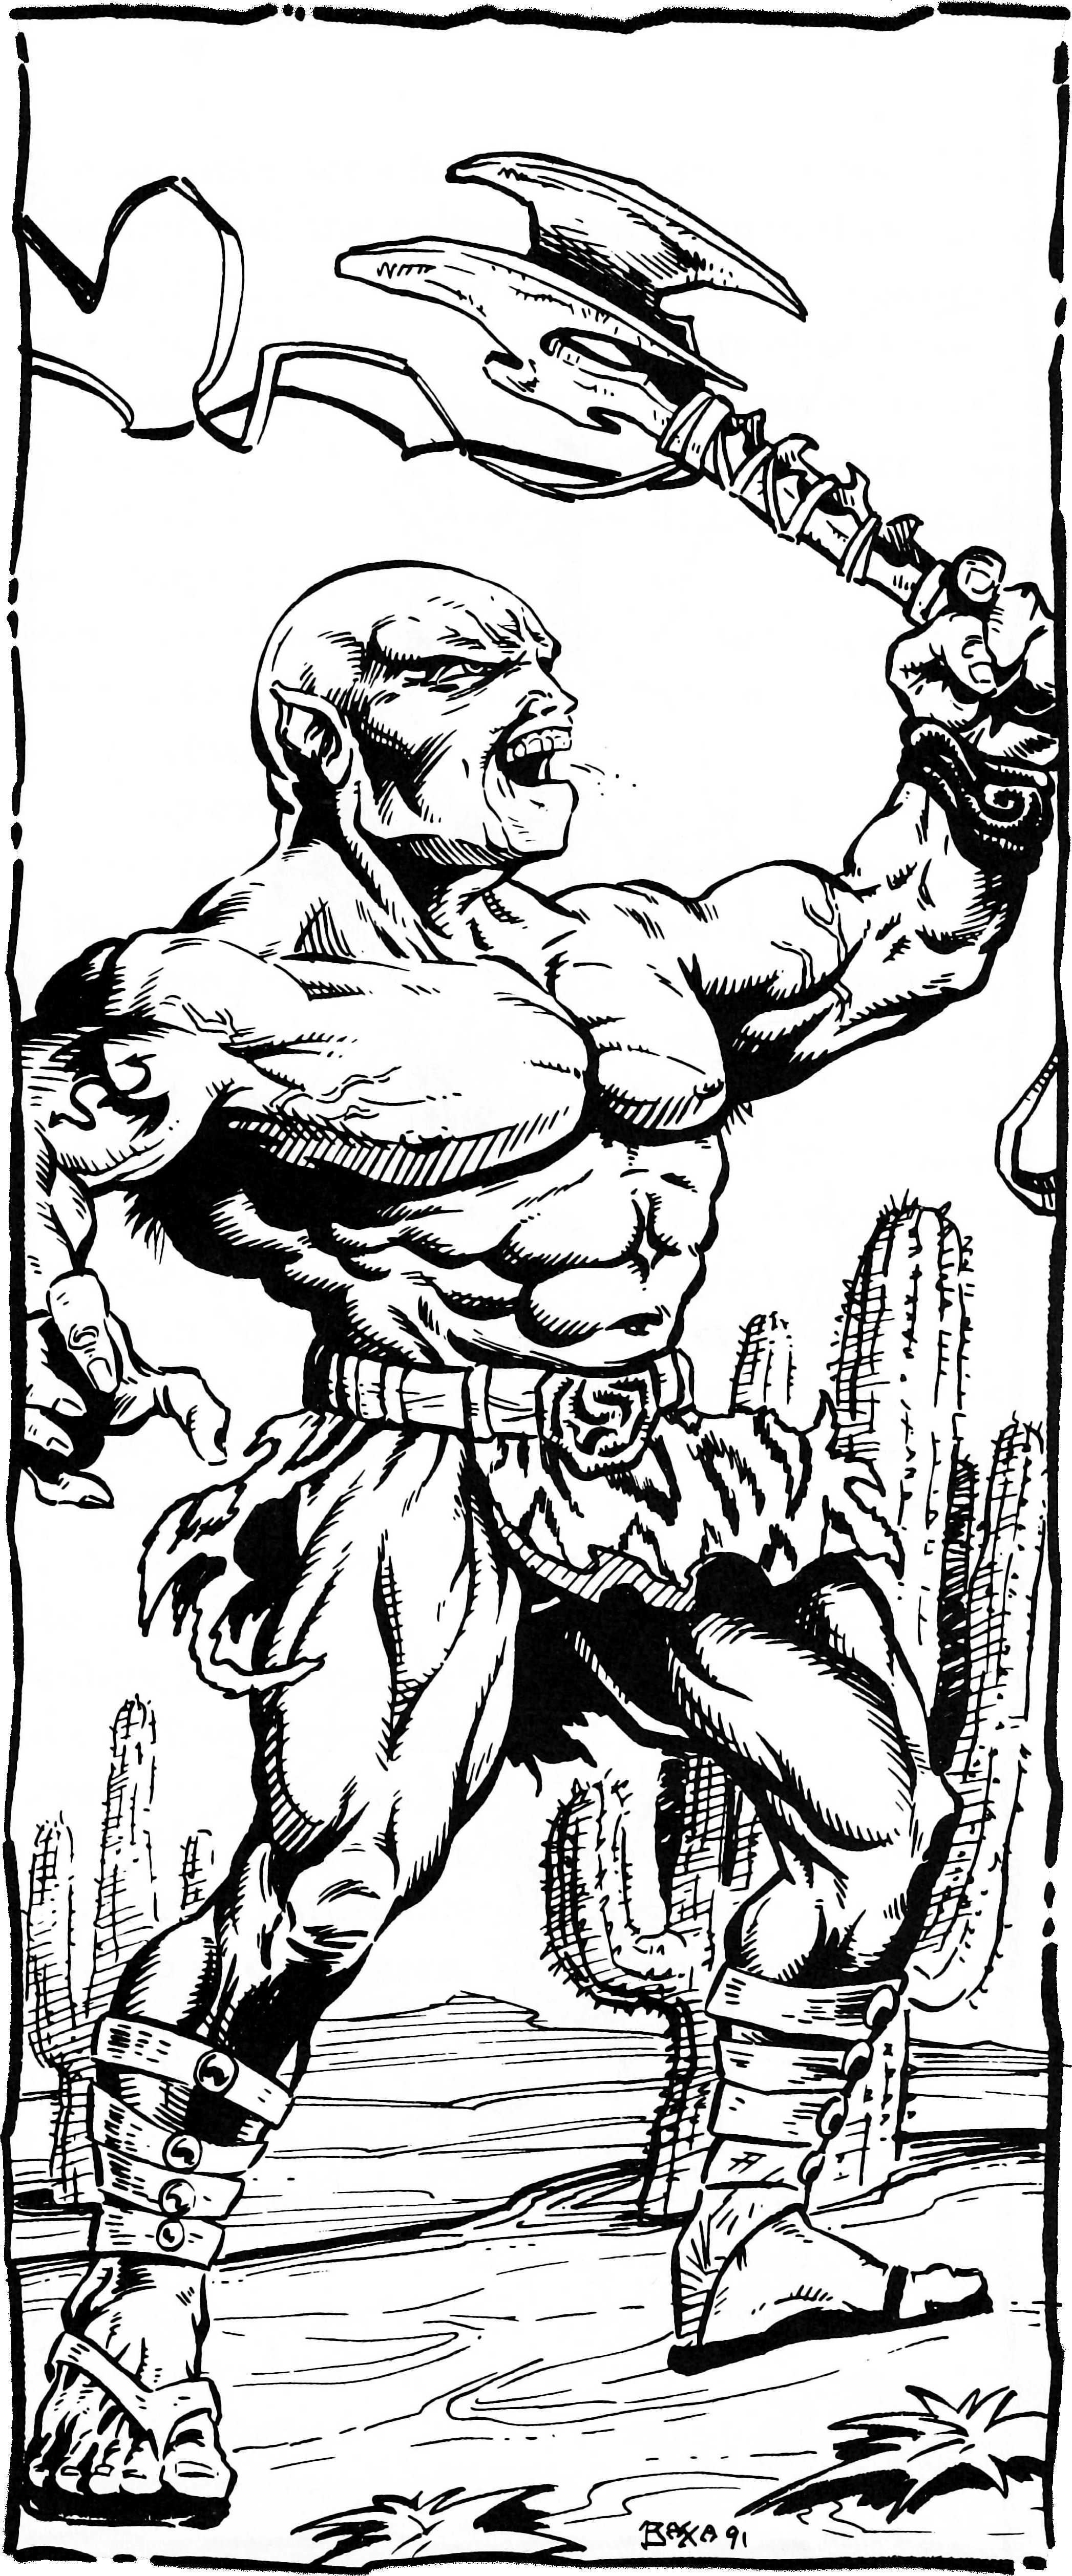
\includegraphics[width=\columnwidth]{images/mul-1.png}
\WOTC
\end{figure}

Born from the unlikely parentage of dwarves and humans, muls combine the height and adaptable nature of humans with the musculature and resilience of dwarves. Muls enjoy traits that are uniquely their own, such as their robust metabolism and almost inexhaustible capacity for work. The hybrid has disadvantages in a few areas as well: sterility, and the social repercussions of being created for a life of slavery. Humans and dwarves are not typically attracted to each other. The only reason that muls are so common in the Tablelands is because of their value as laborers and gladiators: slave-sellers force-breed humans and dwarves for profit. While mul-breeding practices are exorbitantly lucrative, they are often lethal to both the mother and the baby. Conception is difficult and impractical, often taking months to achieve. Even once conceived, the mul takes a full twelve months to carry to term; fatalities during this period are high. As likely as not, anxious overseers cut muls from the dying bodies of their mothers.

\textbf{Personality:} All gladiators who perform well in the arenas receive some degree of pampered treatment, but muls receive more pampering than others. Some mul gladiators even come to see slavery as an acceptable part of their lives. However, those that acquire a taste of freedom will fight for it. Stoic and dull to pain, muls are not easily intimidated by the lash. Masters are loath to slay or maim a mul who tries repeatedly to escape, although those who help the mul's escape will be tormented in order to punish the mul without damaging valuable property. Once a mul escapes or earns his freedom, slavery remains a dominant part of his life. Most muls are heavily marked with tattoos that mark his ownership, history, capabilities and disciplinary measures. Even untattooed muls are marked as a potential windfall for slavers: it is clearly cheaper to ``retrieve'' a mul who slavers can claim had run away, than to start from scratch in the breeding pits.

\textbf{Physical Description:} Second only to the half-giant, the mul is the strongest of the common humanoid races of the tablelands. Muls grow as high as 2.1 meters, weighing upwards of 125 kilograms, but carry almost no fat at all on their broad muscular frames. Universal mul characteristics include angular, almost protrusive eye ridges, and ears that point sharply backwards against the temples. Most muls have dark copper-colored skin and hairless bodies.

\textbf{Relations:} Most mul laborers master the conventions of slave life, figuring out through painful experience who can be trusted and who cannot. (Muls learn from their mistakes in the slave pits to a greater extent than other races not because they are cleverer, but because unlike slaves of other races they tend to survive their mistakes, while other slave races are less expensive and therefore disposable. Only the most foolish and disobedient mul would be killed. Most masters will sell a problem mul slave rather than kill him.) Their mastery of the rules of slave life and their boundless capacity for hard work allows them to gain favor with their masters and reputation among their fellow slaves.

\textbf{Alignment:} Muls tend towards neutrality with respect to good and evil, but run the gamut with respect to law or chaos. Many lawful muls adapt well to the indignities of slavery, playing the game for the comforts that they can win as valued slaves. A few ambitious lawful muls use the respect won from their fellow-slaves to organize rebellions and strike out for freedom. Chaotic muls, on the other hand, push their luck and their value as slaves to the breaking point, defying authority, holding little fear for the lash.

\textbf{Mul Lands:} As a collective group, muls have no lands to call their own. Occasionally, escaped muls band together as outlaws and fugitives, because of their common ex-slave backgrounds, and because their mul metabolism makes it easier for them to survive as fugitives while other races cannot keep up. Almost without exception, muls are born in the slave pits of the merchants and nobles of the city-states. Most are set to work as laborers, some as gladiators, and fewer yet as soldier-slaves. Very few earn their freedom, a greater number escape to freedom among the tribes of ex-slave that inhabit the wastes.

\textbf{Magic:} Muls dislike what they fear, and they fear wizards. They also resent that a wizard's power comes from without, with no seeming effort on the wizard's part, while the mul's power is born of pain and labor. Mul wizards are unheard of.

\textbf{Psionics:} Since most slave owners take steps to ensure that their property does not get schooled in the Way, it is rare for a mul to receive any formal training. Those that get this training tend to excel in psychometabolic powers.

\textbf{Religion:} Even if muls were to create a religion of their own, as sterile hybrids, they would have no posterity to pass it on to. Some cities accept muls as templars. Mul clerics tend to be drawn towards the strength of elemental earth.

\textbf{Language:} Muls speak the Common tongue of slaves, but those favored muls that stay in one city long enough before being sold to the next, sometimes pick up the city language. Because of their tireless metabolism, muls have the capacity to integrate with peoples that other races could not dream of living with, such as elves and Thri-kreen.

\textbf{Names:} Muls sold as laborers will have common slave names. Muls sold as gladiators will often be given more striking and exotic names. Draji names (such as Atlalak) are often popular for gladiators, because of the Draji reputation for violence. Masters who change their mul slaves' professions usually change their names as well, since it is considered bad form to have a gladiator with a farmer's name, and a dangerous incitement of slave rebellions to give a common laborer the name of a gladiator.

\textbf{Adventurers:} Player character muls are assumed to have already won their freedom. Most freed mul gladiators take advantage of their combat skills, working as soldiers or guards. Some turn to crime, adding rogue skills to their repertoire. A few muls follow other paths, such as psionics, templar orders or elemental priesthoods.

\subsection{Mul Society}
Muls have no racial history or a separate culture. They are sterile and cannot reproduce, preventing them from forming family groups and clans. The vast majority of muls are born in slavery, through breeding programs. Often the parents resent their roles in the breeding program and shun the child, leaving the mul to a lonely, hard existence. The taskmaster's whip takes the place of a family. For these reasons, many muls never seek friends or companionship, and often have rough personalities with tendencies towards violence.

The mul slave trade is very profitable, and thus the breeding programs continue. A slave trader can make as much on the sale of a mul as he could with a dozen humans. As slaves, a mul has his profession selected for him and is given extensive training as he grows.

Mul gladiators are often very successful, and win a lot of money for their owners. Highly successful gladiators are looked after by their owners, receiving a large retinue of other slaves to tend to their whims and needs. This has lead to the expression, ``pampered like a mul,'' being used often by the common folk.

Muls not trained as gladiators are often assigned to hard labor and other duties that can take advantage of the mul's hardy constitution and endurance.

\subsection{Roleplaying Suggestions}
Born to the slave pens, you never knew love or affection; the taskmaster's whip took the place of loving parents. As far as you have seen, all of life's problems that can be solved are solved by sheer brute force. You know to bow to force when you see it, especially the veiled force of wealth, power and privilege. The noble and templar may not look strong, but they can kill a man with a word. You tend towards gruffness. In the slave pits, you knew some muls that never sought friends or companionship, but lived in bitter, isolated servitude. You knew other muls who found friendship in an arena partner or co-worker. You are capable of affection, trust and friendship, but camaraderie is easier for you to understand and express - warriors slap each other on the shoulder after a victory, or give their lives for each other in battle. You don't think of that sort of event as ``friendship'' - it just happens.

\subsection{Mul Racial Traits}
\begin{itemize*}
    \item +4 Strength, +2 Constitution, $-2$ Charisma: Combining the human height with the Dwarven musculature, muls end up stronger than either parent race, but their status as born-to-be slaves makes them insecure in their dealings with others.
    \item Humanoid (dwarf): Muls are humanoid creatures with the dwarf subtype.
    \item Medium: As Medium creatures, muls have no bonuses or penalties due to size.
    \item Mul base land speed is 9 meters.
    \item Darkvision: Muls can see in the dark up to 9 meters. Darkvision is black and white only, but is otherwise like normal sight, and muls can function just fine with no light at all.
    \item Tireless: Muls get a +4 racial bonus to checks for performing a physical action that extends over a period of time (running, swimming, holding breath, and so on). This bonus stacks with the \feat{Endurance} feat. This bonus may also be applied to savings throws against spells and magical effects that cause weakness, fatigue, exhaustion or enfeeblement.
    \item Extended Activity: Muls may engage in up to 12 hours of hard labor or forced marching without suffering from fatigue.
    \item Dwarven Blood: For all effects related to race, a mul is considered a dwarf. Muls, for example, are just as vulnerable to effects that affect dwarves as their dwarf ancestors are, and they can use magic items that are only usable by dwarves.
    \item Nonlethal Damage Resistance 1/--. Muls are difficult to subdue, and do not notice minor bruises, scrapes, and other discomforts that pain creatures of other races.
    \item Favored Class: Gladiator. A multiclass mul's gladiator class does not count when determining whether he takes an experience point for multiclassing.
    \item Automatic Language: Common. Bonus Languages: Dwarven, Elven, Gith, and Giant.
    \item Level Adjustment: +1. As a hybrid half-race, muls are considerably more powerful than either of their parent races, thus they gain levels more slowly.
\end{itemize*}